\chapter{\textbf{Metodologia de Pesquisa}} % Este comando é utilizado para criar capítulos
\sloppy % Corrige estouro de linhas

\section{Web Service Restful e Aplicativo}

Para a construção do Web Service Restful e do aplicativo foi utilizado como referência o modelo aplicado na disciplina de Laboratório de Engenharia de Software do curso de Sistemas de Informação do Ifes Campus Cachoeiro, baseado no \textit{Rational Unified Process} (RUP), representado na figura \ref{figura:rup}.

\begin{figure}[h]
	\caption{Processo de desenvolvimento de \textit{software} baseado no RUP.}
	\centering % para centralizarmos a figura
	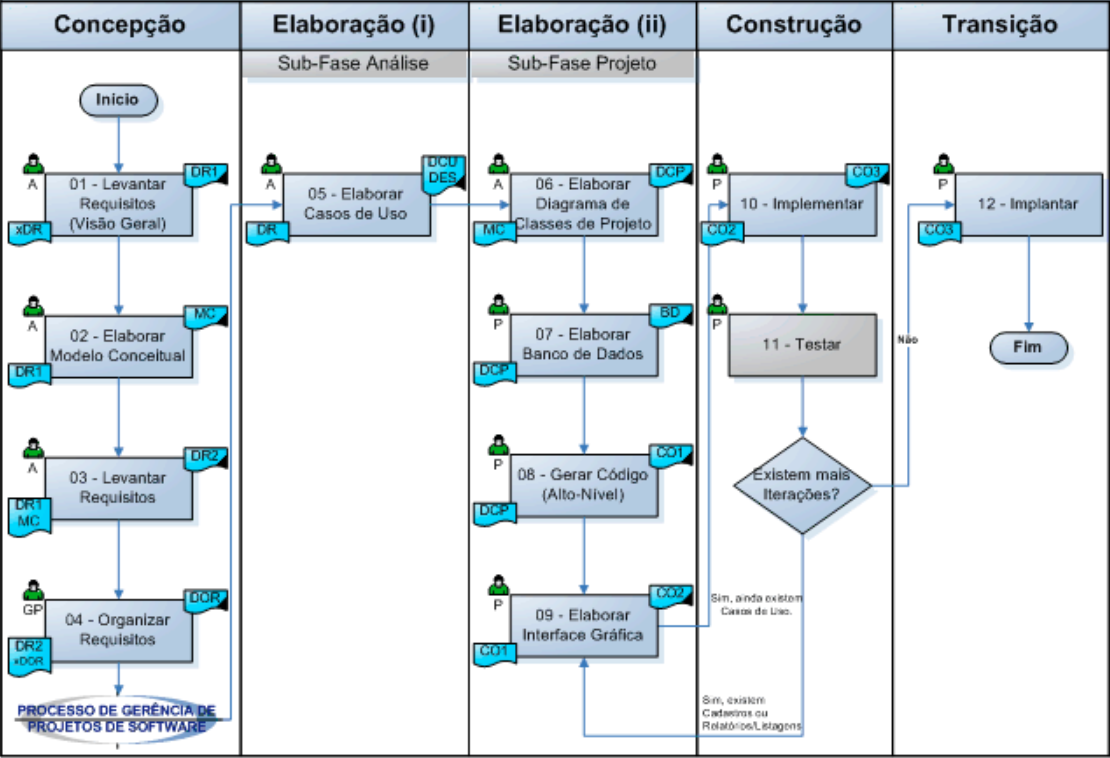
\includegraphics[width=16cm]{resources/pds_rup.png} % leia abaixo
	\label{figura:rup}	
	\caption*{Fonte: \citeonline{rupLes}.}
\end{figure}

Para tal, os seguintes passos descritos no modelo (figura \ref{figura:rup}) foram executados para a elaboração dos \textit{sofwares}:

\begin{enumerate}
   \item Levantar Requisitos (Visão Geral): identificar descrever de forma geral o funcionamento do aplicativo e suas principais funções;
   \item Elaborar modelo conceitual: identificar classes e relacionamentos concernentes ao domínio (nesta fase não se faz necessário a inclusão dos atributos nas classes);
   \item Levantar Requisitos: elaborar documento de requisitos contendo o detalhamento de todas as funcionalidades do aplicativo;
   \item Organizar Requisitos: elaborar documento de organização de requisitos separando todos os requisitos em processos de negócios e relatórios/listagens;
   \item Elaborar banco de dados: 
   \item Elaborar interface gráfica: estruturar todas as telas do aplicativo;
   \item Implementar: codificar as classes necessárias para implementação das funcionalidades de processos de negócio e listagens;
   \item Testar: realizar testes de todas as funcionalidades implementadas;
   \item Implantar: gerar o arquivo instalável do aplicativo (APK) e instalar o \textit{webservice} no servidor de produção;
\end{enumerate}

\section{Módulo de Recomendação}

Para a construção do módulo de recomendação do aplicativo foi utilizado a biblioteca Weka para realizar o treinamento da rede e extrair os resultados do mesmo. Para tanto, a biblioteca utiliza um arquivo do tipo ARFF para descrever os os atributos, as possibilidades de classificação e os respectivos exemplos de classificação utilizados no treinamento em questão. Sua estrutura básica é representada na figura \ref{figura:arff}.

\begin{figure}[h]
	\caption{Sintaxe básica de um arquivo de treinamento utilizado pelo Weka.}
	\centering % para centralizarmos a figura
	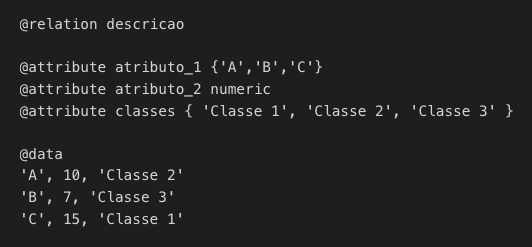
\includegraphics[width=12cm]{resources/arff.png} % leia abaixo
	\label{figura:arff}	
	\caption*{Fonte: O Autor.}
\end{figure}

\break

\section{Ambiente de desenvolvimento}

As seguintes ferramentas e \textit{softwares} foram utilizados no processo de desenvolvimento:

\begin{itemize}
    \item Banco de Dados Oracle (versão 11g);
    \item Java SE \textit{Development Kit} (versão 8 update 221);
    \item Ionic \textit{Framework} (versão 4);
    \item Servidor Web Payara (versão 5.191);
    \item Netbeans IDE (versão 11.1);
    \item Visual Studio Code (versão 1.39.1);
    \item Postman (versão 7.2);
\end{itemize}